%==============================================================================
% Supplementary material for the SIMTiX TVLSI manuscript (simtix_tvlsi.tex).
% Build after the paper (references to it come from simtix_tvlsi.aux via xr):
%   pdflatex simtix_tvlsi && pdflatex simtix_tvlsi_supp && pdflatex simtix_tvlsi_supp
% Parts: supp_figs.tex (ratio figures moved from the paper), supp_lanes.tex (lane
% scaling in full), supp_evalmem.tex (memory-system measurements of the v2 design).
%==============================================================================
\documentclass[journal]{IEEEtran}

\usepackage{cite}
\usepackage{amsmath,amssymb}
\usepackage{graphicx}
\usepackage{booktabs}
\usepackage{xcolor}
\usepackage{xr-hyper}
\usepackage[hidelinks]{hyperref}
\externaldocument[P-]{simtix_tvlsi}

\graphicspath{{../figs/}}
\newcommand{\Fmax}{$F_{\max}$}
\renewcommand{\thesection}{S\arabic{section}}
\renewcommand{\thefigure}{S\arabic{figure}}
\renewcommand{\thetable}{S\Roman{table}}
\usepackage{array}
\usepackage{multirow}
\usepackage{url}

\begin{document}

\title{Supplementary Material for ``SIMTiX: A Compact RISC-V SIMT Accelerator With
Line-Aggregated Atomic Operations for FPGA Systems-on-Chip''}
\author{Krishna~Gorai and Bikram~Paul}
\markboth{IEEE Transactions on Very Large Scale Integration (VLSI) Systems}%
{Gorai and Paul: SIMTiX, Supplementary Material}
\maketitle

This document holds figures and measurements that support the paper but did not fit
its page budget. Tables, figures and sections without the prefix S are those of the
paper.

\section{The Launch and One Warp, Cycle by Cycle}\label{sup:cycles}
Fig.~\ref{fig:fullwave} shows windows of the launch of Fig.~\ref{P-fig:launch} of the
paper with all of their signals, one column per clock cycle: the warp that the spawner
places, that fetch takes and that X issues, with its opcode; the eight warp slots; the
L1's requests and tag lookups; the five AXI4 channels; and the register-file writes,
over cycles 0 to 23, 44 to 67 and 96 to 119. Figs.~\ref{P-fig:wavea}
to~\ref{P-fig:wavec} of the paper show the signals that matter in each window.
Fig.~\ref{fig:pipechart} follows every instruction of the warp of
Fig.~\ref{P-fig:pipe} of the paper through the pipeline stages: each row is an
instruction and each box a cycle in a stage, from the fetch (F) to the register write
(W), and the time axis leaves out three stretches in which only memory is busy. The
circled numbers mark the waits of the critical path: the load of $y$ waits because the
warp has two loads in flight, the FMA waits for $x$ and $y$, and the store holds the
warp until DDR4 answers the write.

\begin{figure*}[p]
\centering
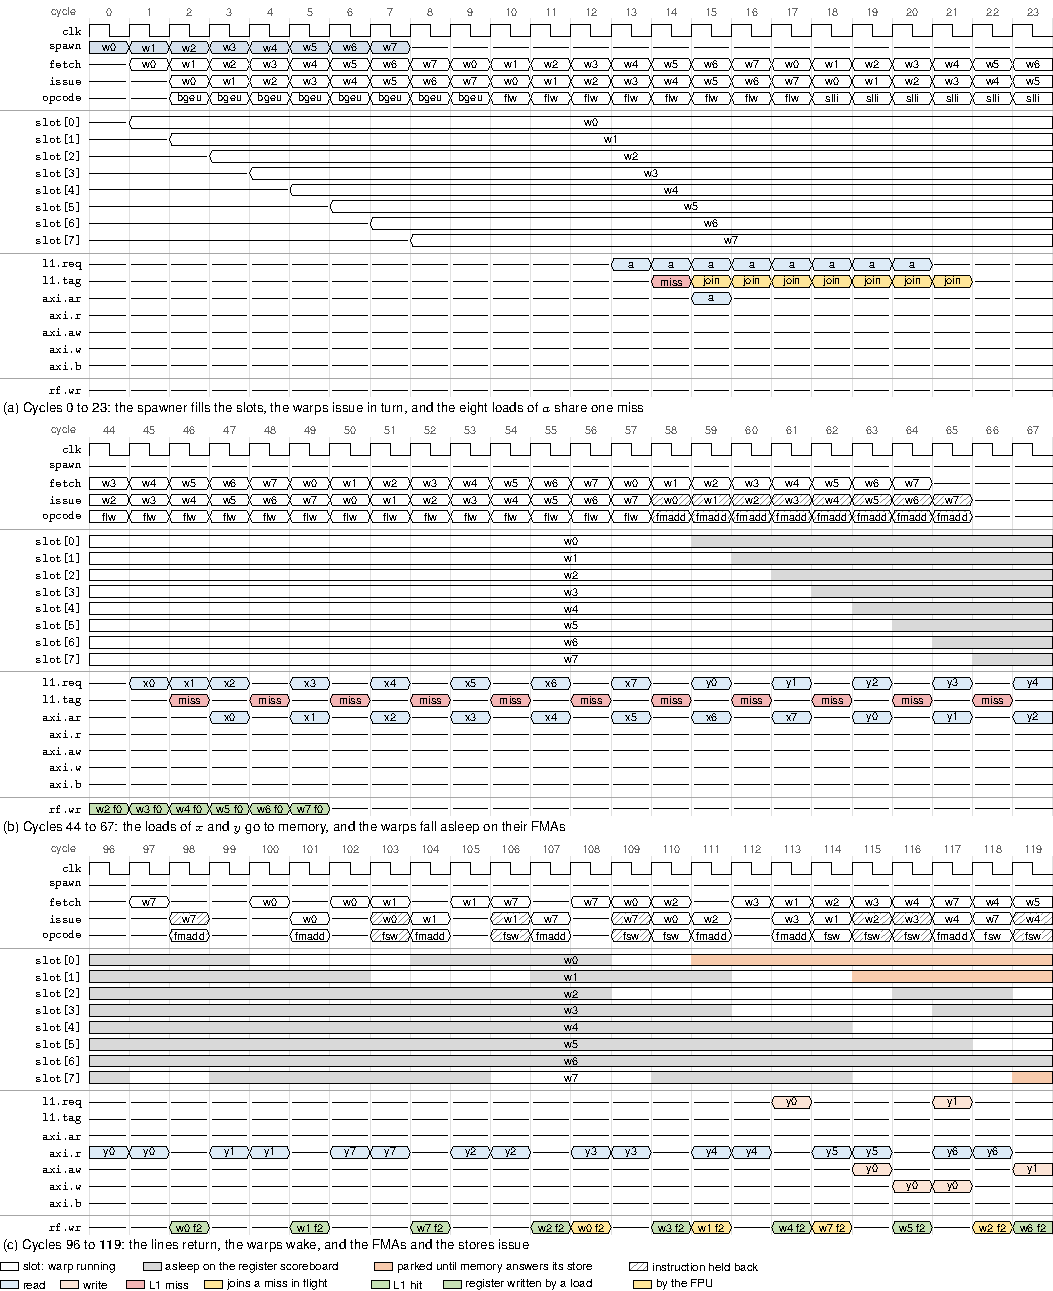
\includegraphics[width=\textwidth]{simtix_launch_wave.pdf}
\caption{Three windows of the launch of Fig.~\ref{P-fig:launch}, all signals, traced on
the RTL.}
\label{fig:fullwave}
\end{figure*}

\begin{figure*}[t]
\centering
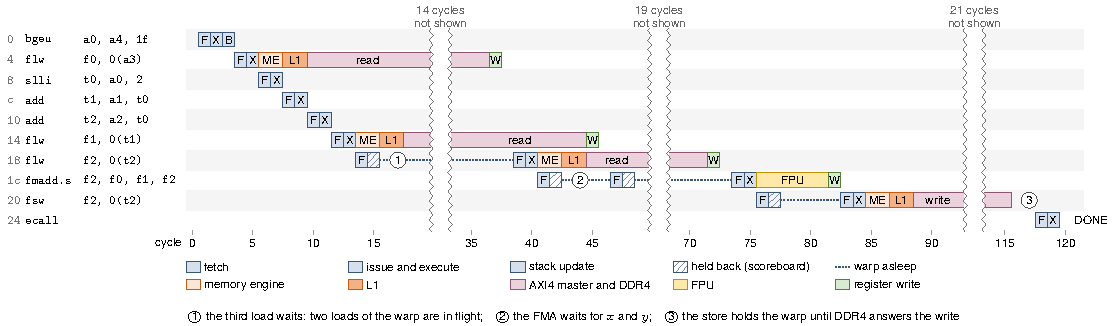
\includegraphics[width=\textwidth]{simtix_pipe.pdf}
\caption{Every instruction of the warp of Fig.~\ref{P-fig:pipe} through the pipeline
stages, traced on the RTL.}
\label{fig:pipechart}
\end{figure*}

\section{Divergence of One Warp}\label{sup:div}
\begin{figure*}[t]
\centering
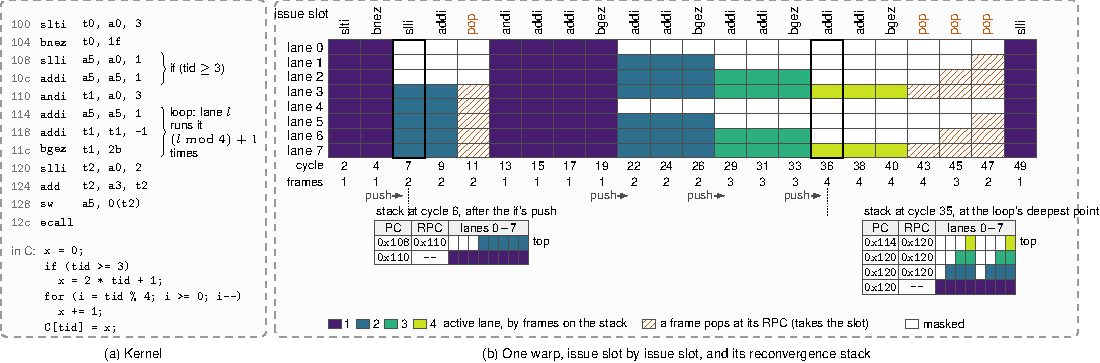
\includegraphics[width=\textwidth]{simtix_div.pdf}
\caption{Divergence and reconvergence of one warp, traced on the RTL.}
\label{fig:div}
\end{figure*}

Fig.~\ref{fig:div} traces one warp on the RTL through the kernel of
Fig.~\ref{fig:div}(a), given in C and as the RV32 instructions at their PCs: a
one-sided \texttt{if} and a loop whose trip count differs per lane. In
Fig.~\ref{fig:div}(b) each column is one issue slot of the warp and each row a
lane: a filled cell is an active lane, coloured by the number of frames on the stack, a
white cell a masked lane, and a hatched cell a lane of a frame that pops. The row above
the grid names the instruction of each slot, and the rows below give its cycle, the
number of frames and the pushes. The two tables give the PC, RPC and lanes of every
frame at two points, with the top frame marked and -- for the bottom frame, which has
no RPC. The \texttt{bnez} of
cycle 4 is taken by lanes 0 to 2, so stage B pushes a frame of lanes 3 to 7 with the
branch target 0x110 as RPC, and the frame below waits at 0x110 with all eight lanes
(first table). Lanes 3 to 7 run the body in cycles 7 and 9; in cycle 11 the top frame's
PC reaches its RPC and the frame pops, which takes the issue slot, and the warp goes on
with all lanes. In the loop, lane $l$ runs $(l\bmod 4)+1$ iterations. The
\texttt{bgez} that ends the first iteration keeps lanes 1 to 3 and 5 to 7 in the loop
and pushes them, while the frame below waits at the exit 0x120; the second and third
iterations push again, each time without the two lanes that leave, so in cycle 35 the
stack holds four frames (second table), one per distinct trip count, as
Theorem~\ref{P-thm:stack} allows. In the fourth iteration the last two lanes leave
together, a uniform branch that pushes nothing; the three pushed frames then pop in
cycles 43, 45 and 47, and in cycle 49 the warp runs with all eight lanes again. Up to
this point the warp takes 22 issue slots for its 18 instructions, and its lanes are
active in 102 of the 144 lane slots of these instructions, a lane utilization of 0.71
(Section~\ref{P-sec:evallanes}).

\section{Four Warps Under the Issue Rules}\label{sup:lat4}
\begin{figure*}[t]
\centering
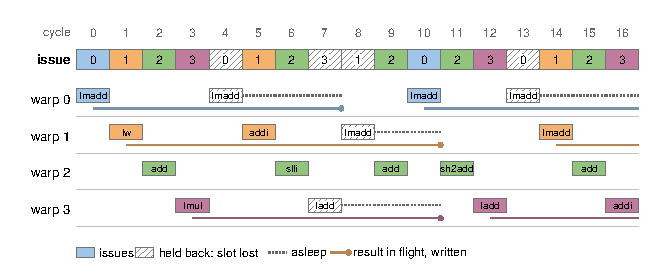
\includegraphics{simtix_lat_a.pdf}
\caption{Four warps under the issue rules (FPU result written seven cycles after issue;
load latency schematic).}
\label{fig:lat4}
\end{figure*}

Fig.~\ref{fig:lat4} shows four warps under the issue rules of Section~\ref{P-sec:arch} of the paper, with the FPU result written
seven cycles after issue and a schematic load latency: warp 0 runs dependent FMAs
(\texttt{fmadd}); warp 1 a load (\texttt{lw}), an \texttt{addi} and two FMAs; warp 2
integer code (\texttt{add}, \texttt{slli} and the Zba shift-and-add \texttt{sh2add});
and warp 3 a multiply (\texttt{fmul}), two adds (\texttt{fadd}) and an \texttt{addi}.
The top row (\texttt{issue}) gives the warp in X in each cycle, and each warp's row its
issues, held-back cycles, sleep and results in flight. In cycle 4 warp 0's second FMA
finds the first one's result still in the FPU, so it is held back, its slot is lost
and warp 0 sleeps until the write in cycle 7; warps 3 and 1 lose cycles 7 and 8 in the
same way, while the integer instructions of warp 2 and of woken warps take the other
slots, and warp 1 issues its \texttt{addi} while its load is in flight. Four of the 17
slots are lost. As a cycle model, these rules reproduce the RTL's issue trace of a
four-warp test kernel cycle by cycle.

\section{Execution Time and Cycles of the Machines}\label{sup:ratios}
\begin{table*}[t]
\caption{Run Times on the Applications and Rodinia}
\label{tab:rodinia}
\centering\footnotesize
\setlength{\tabcolsep}{3.2pt}
\begin{tabular*}{\textwidth}{@{\extracolsep{\fill}}llrrrrrrrrrrr@{}}
\toprule
 & & SIMTiX & \multicolumn{2}{c}{CVA6} & \multicolumn{2}{c}{Ara} & \multicolumn{2}{c}{Vortex}
 & \multicolumn{2}{c}{FGPU} & \multicolumn{2}{c}{Cortex-A53}\\
\cmidrule(lr){3-3}\cmidrule(lr){4-5}\cmidrule(lr){6-7}\cmidrule(lr){8-9}\cmidrule(lr){10-11}\cmidrule(lr){12-13}
Benchmark & Input & Time (ms) & Time (ms) & Ratio & Time (ms) & Ratio & Time (ms) & Ratio
 & Time (ms) & Ratio & Time (ms) & Ratio\\
\midrule
\multicolumn{13}{@{}l}{\emph{Applications of Table~\ref{tab:board}}}\\
GEMM-RB    & $256^3$                       & 37.8    & 3,689.7   & 97.7 & 77.4     & 2.05 & 198.2    & 5.25 & 296.5 & 7.85 & 169.6    & 4.49\\
SpMV-Z     & 65,536 rows                   & 19.3    & 362.3     & 18.7 & 313.2    & 16.2 & 46.2     & 2.39 & 200.3 & 10.4 & 18.3     & 0.95\\
CNN        & $128^2$, 16-32-32 channels    & 290.7   & 27,266.5  & 93.8 & 1,581.3  & 5.44 & 2,066.4  & 7.11 & 892.0 & 3.07 & 1,191.9  & 4.10\\
Mandelbrot & $1024^2$, 256 iterations      & 1,019.7 & 11,142.5  & 10.9 & 4,553.5  & 4.47 & 5,324.0  & 5.22 & 858.7 & 0.84 & 846.8    & 0.83\\
\midrule
\multicolumn{13}{@{}l}{\emph{Rodinia}}\\
pathfinder & 100 rows, 100,000 columns   & 250.5   & 4,428.8   & 17.7 & 421.2    & 1.68 & 960.9    & 3.84 & 650.0 & 2.60 & 97.2     & 0.39\\
backprop   & 2$^{19}$ inputs, 16 hidden    & 299.2   & 5,729.0   & 19.1 & 3,055.4  & 10.2 & 1,008.8  & 3.37 & 791.4 & 2.64 & 214.2    & 0.72\\
bfs        & graph65536                    & 36.7    & 299.8     & 8.17 & 794.1    & 21.7 & 126.8    & 3.46 & 138.3 & 3.77 & 21.9     & 0.60\\
hotspot    & $512^2$, 2 iterations         & 33.6    & 553.1     & 16.5 & 45.3     & 1.35 & 103.0    & 3.07 & 60.4 & 1.80 & 21.0     & 0.63\\
hotspot    & $1024^2$, 2 iterations        & 134.2   & 2,475.0   & 18.4 & 172.8    & 1.29 & 411.2    & 3.06 & 241.4 & 1.80 & 85.5     & 0.64\\
nn         & 42,764 records                & 15.3    & 24.4      & 1.59 & 8.9      & 0.58 & 4.8      & 0.31 & 2.1 & 0.14 & 1.0      & 0.07\\
hotspot3D  & $512^2\times8$, 100 iterations & 9,449.6 & 491,642.8 & 52.0 & 20,528.6 & 2.17 & 21,504.5 & 2.28 & 22,239.8 & 2.35 & 16,522.7 & 1.75\\
gaussian   & $1024\times1024$              & 4,965.0 & 104,642.3 & 21.1 & 10,176.9 & 2.05 & 6,064.0  & 1.22 & 9,923.2 & 2.00 & 3,916.4  & 0.79\\
kmeans     & kdd\_cup, $k=5$, 37 iterations & 31,810.0 & 726,014.0 & 22.8 & 56,290.0 & 1.77 & 64,442.3 & 2.03 & 63,549.7 & 2.00 & 28,064.9 & 0.88\\
\midrule
\multicolumn{13}{@{}l}{\emph{Geometric mean of the ratio}}\\
\multicolumn{3}{@{}l}{Rodinia, time} & & 14.6 & & 2.62 & & 1.98 & & 1.67 & & 0.56\\
\multicolumn{3}{@{}l}{Rodinia, clock cycles} & & 9.97 & & 1.79 & & 2.15 & & 2.71 & & ---\\
\multicolumn{3}{@{}l}{All twelve, time} & & 19.9 & & 3.32 & & 2.63 & & 2.20 & & 0.85\\
\multicolumn{3}{@{}l}{All twelve, clock cycles} & & 13.6 & & 2.27 & & 2.85 & & 3.57 & & ---\\
\bottomrule
\end{tabular*}
\end{table*}

\begin{table*}[t]
\caption{Run Times on RiVEC}
\label{tab:rivec}
\centering\footnotesize
\setlength{\tabcolsep}{3.2pt}
\begin{tabular*}{\textwidth}{@{\extracolsep{\fill}}llrrrrrrrrrrr@{}}
\toprule
 & & SIMTiX & \multicolumn{2}{c}{CVA6} & \multicolumn{2}{c}{Ara} & \multicolumn{2}{c}{Vortex}
 & \multicolumn{2}{c}{FGPU} & \multicolumn{2}{c}{Cortex-A53}\\
\cmidrule(lr){3-3}\cmidrule(lr){4-5}\cmidrule(lr){6-7}\cmidrule(lr){8-9}\cmidrule(lr){10-11}\cmidrule(lr){12-13}
Application & Input & Time (ms) & Time (ms) & Ratio & Time (ms) & Ratio & Time (ms) & Ratio
 & Time (ms) & Ratio & Time (ms) & Ratio\\
\midrule
axpy         & 2,097,152 elements             & 31.5 & 513.4 & 16.3 & 50.7 & 1.61 & 179.2 & 5.69 & 103.1 & 3.27 & 25.0 & 0.80 \\
matmul       & $512^3$, RiVEC data            & 300.3 & 65,174.2 & 217 & 14,918.2 & 49.7 & 1,562.4 & 5.20 & 2,840.4 & 9.46 & 2,152.8 & 7.17 \\
spmv         & poisson3Db, $A^{\mathsf T}x$   & 79.2 & 1,211.9 & 15.3 & 567.1 & 7.16 & 173.6 & 2.19 & 1,152.7 & 14.6 & 52.8 & 0.67 \\
jacobi-2d    & $256^2$, 2,000 steps           & 10,116.6 & 145,978.7 & 14.4 & 19,324.5 & 1.91 & 36,713.8 & 3.63 & 18,790.4 & 1.86 & 4,461.7 & 0.44 \\
pathfinder   & $1024\times2048$, 100 runs     & 5,556.7 & 116,179.1 & 20.9 & 8,907.6 & 1.60 & 22,044.9 & 3.97 & 14,464.1 & 2.60 & 2,473.0 & 0.45 \\
blackscholes & 65,536 options, 100 runs       & 9,328.3 & 45,462.0 & 4.87 & 5,665.7 & 0.61 & 9,095.9 & 0.98 & 3,420.8 & 0.37 & 3,460.8 & 0.37 \\
lavaMD       & $10^3$ boxes of 96 particles   & 15,868.0 & 268,712.8 & 16.9 & 159,494.0 & 10.1 & 69,823.7 & 4.40 & 13,980.1 & 0.88 & 23,438.5 & 1.48 \\
\midrule
\multicolumn{13}{@{}l}{\emph{Geometric mean of the ratio}}\\
\multicolumn{3}{@{}l}{Time} & & 20.1 & & 3.76 & & 3.27 & & 2.55 & & 0.88\\
\multicolumn{3}{@{}l}{Clock cycles} & & 13.8 & & 2.59 & & 3.53 & & 4.16 & & ---\\
\bottomrule
\end{tabular*}
\end{table*}

Figs.~\ref{fig:rodinia} and~\ref{fig:rivec} give, for every Rodinia benchmark and
RiVEC application at its largest input, the execution time and the clock cycles of
SIMTiX with 16 and with eight lanes, CVA6, Ara, Vortex and FGPU, each at its own clock:
the eight-lane and the other machines' values from Tables~\ref{tab:rodinia}
and~\ref{tab:rivec}, the 16-lane values from the board runs of
Section~\ref{sup:lanes16} at 100~MHz; FGPU's cycles are its time times its clock. Fig.~\ref{fig:mach_time} gives the execution time of every
machine, the eight- and 16-lane SIMTiX included, on all twelve applications of
Table~\ref{tab:board}, Rodinia and RiVEC at their largest inputs, the integer
benchmarks that Fig.~\ref{P-fig:mach_heatmap} of the paper leaves out among them; Ara
gives wrong results on the MLP and Smith-Waterman.
In Figs.~\ref{fig:rodinia} and~\ref{fig:rivec} each benchmark has one bar per machine on
a log axis. The 16-lane SIMTiX is the fastest of the six designs on 12 of the 15
benchmarks, and the eight-lane design on RiVEC's spmv, a gather that the 16-lane line of
64 bytes slows (Section~\ref{P-sec:lanes16} of the paper). FGPU, with a divide and
square-root unit per lane, leads on nn and blackscholes; on lavaMD, where it is faster
than the eight-lane design, the 16-lane design takes 0.65 of its time. The A53, which
Tables~\ref{tab:rodinia} and~\ref{tab:rivec} and Fig.~\ref{fig:mach_time} include, is
faster than the eight-lane SIMTiX on every Rodinia benchmark but hotspot3D. In Fig.~\ref{fig:mach_time} each row is a benchmark and each column a
machine, and the colour and the number give the time in milliseconds on a log scale.
Section~\ref{P-sec:decomp} of the paper splits the time ratios into clock, width and
efficiency.

\begin{figure*}[t]
\centering
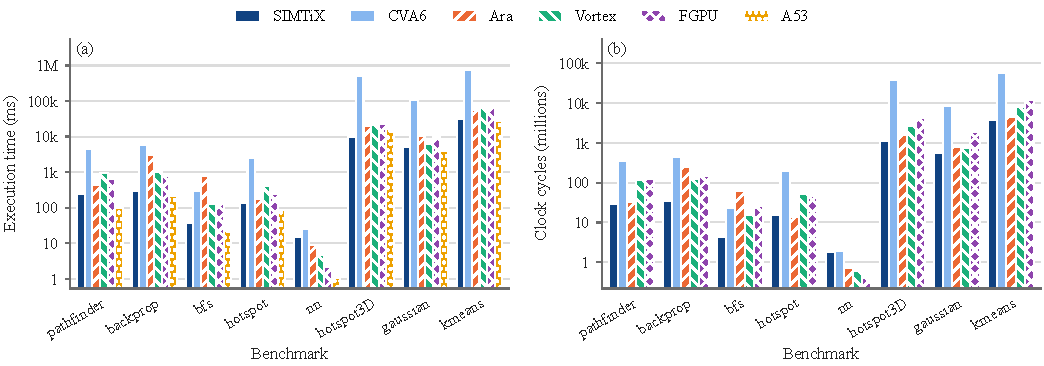
\includegraphics[width=\textwidth]{rodinia_time.pdf}
\caption{Rodinia on the ZCU102. (a) Execution time. (b) Clock cycles.}
\label{fig:rodinia}
\end{figure*}

\begin{figure*}[t]
\centering
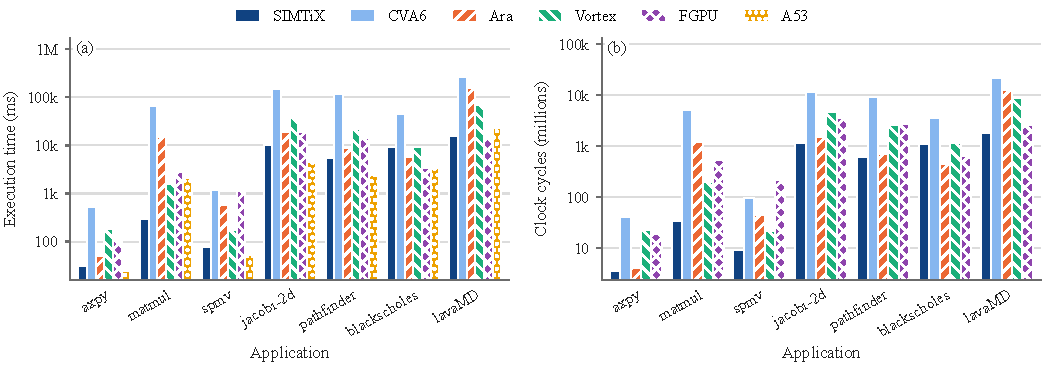
\includegraphics[width=\textwidth]{rivec_time.pdf}
\caption{RiVEC on the ZCU102. (a) Execution time. (b) Clock cycles.}
\label{fig:rivec}
\end{figure*}

\begin{figure*}[t]
\centering
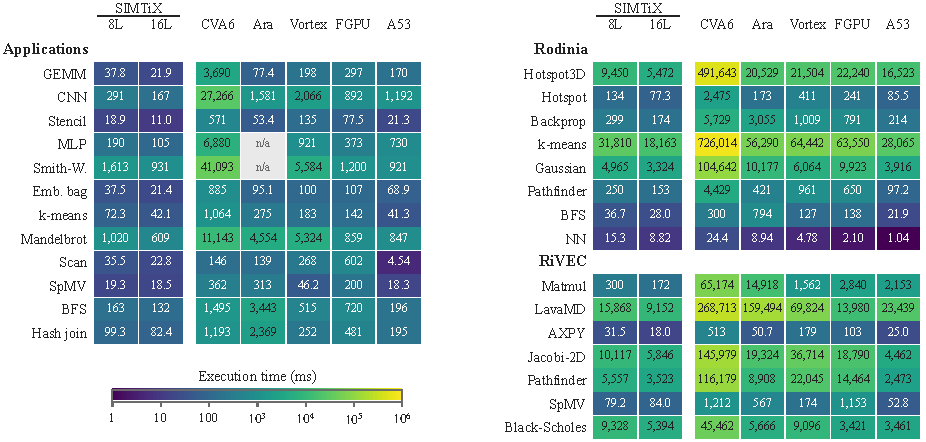
\includegraphics[width=\textwidth]{machines_heatmap_time.pdf}
\caption{Execution time of each machine on the ZCU102.}
\label{fig:mach_time}
\end{figure*}


\section{Applications Against the Cortex-A53}\label{sup:a53}
Table~\ref{tab:board} gives the time of each of the twelve applications on one A53 core
and on SIMTiX, the board power while each computes, and the A53's time and energy
over SIMTiX's, so above 1 favors SIMTiX (Section~\ref{P-sec:evalboard} of the paper).
The A53 runs an ordinary sequential C algorithm built with \texttt{-O2} and with
\texttt{-O3 -mcpu=cortex-a53}, which vectorizes with NEON; the faster build is
\texttt{-O3} for every application but Smith-Waterman, for which it is \texttt{-O2}.
Each application runs at the large input listed in Section~\ref{sup:sim}, and every
output of the accelerator is compared exactly with the A53's. For power, the host reads
the board's 18 INA226 monitors over I$^2$C while each phase repeats for 2~s and sums
the rails. One A53 pass of the MLP takes 730~ms, and the rails are sampled only between
passes; the A53's power on it is within the noise of its few samples, so the table
gives no power or energy for the MLP.

\begin{table}[t]
\caption{SIMTiX Against the Cortex-A53 on the Applications}
\label{tab:board}
\centering\footnotesize
\setlength{\tabcolsep}{3.2pt}
\begin{tabular}{@{}lrrrrrr@{}}
\toprule
 & \multicolumn{2}{c}{Time (ms)} & \multicolumn{2}{c}{Power (W)} & \multicolumn{2}{c}{A53 / SIMTiX}\\
\cmidrule(lr){2-3}\cmidrule(lr){4-5}\cmidrule(lr){6-7}
Application & A53 & SIMTiX & A53 & SIMTiX & Time & Energy\\
\midrule
Hash join       &   195.4 &    99.3 & 3.13 & 4.12 & 1.97 & 1.50\\
CNN             &   381.8 &   290.7 & 3.11 & 4.00 & 1.31 & 1.02\\
GEMM-RB         &    47.2 &    37.8 & 3.17 & 4.22 & 1.25 & 0.94\\
Embedding bag   &    45.4 &    37.5 & 3.12 & 4.05 & 1.21 & 0.94\\
BFS             &   194.6 &   162.9 & 3.13 & 3.88 & 1.19 & 0.96\\
SpMV-Z          &    18.1 &    19.4 & 3.17 & 4.08 & 0.94 & 0.73\\
Mandelbrot      &   845.7 & 1,019.7 & 3.12 & 4.19 & 0.83 & 0.62\\
Smith-Waterman  &   922.1 & 1,613.4 & 3.16 & 3.83 & 0.57 & 0.47\\
k-means-U       &    34.3 &    72.2 & 3.11 & 3.86 & 0.47 & 0.38\\
Stencil-RB      &     8.6 &    18.9 & 3.20 & 4.26 & 0.45 & 0.34\\
MLP             &    55.4 &   189.8 &  --- &  --- & 0.29 & ---\\
Segmented scan  &     4.5 &    35.5 & 3.27 & 3.91 & 0.13 & 0.11\\
\bottomrule
\end{tabular}
\end{table}

\section{Power and Energy per Run}\label{sup:energy}
\begin{figure*}[t]
\centering
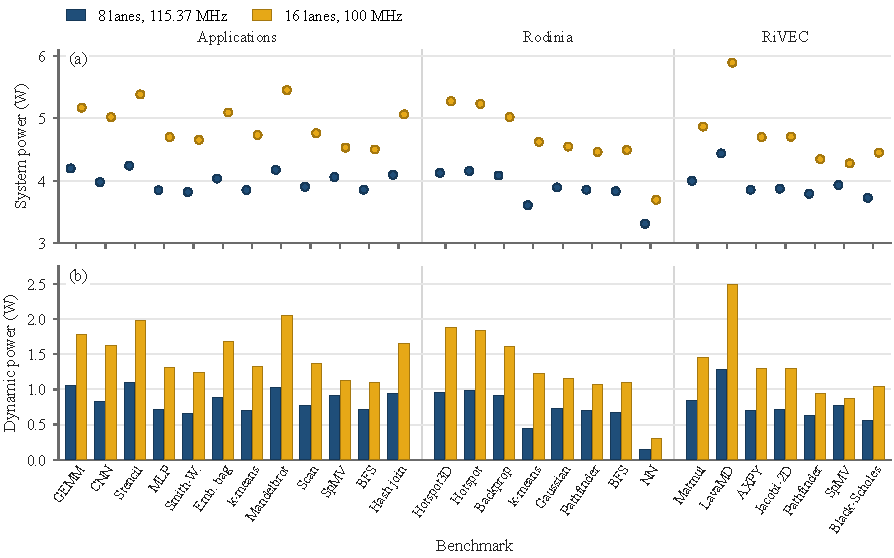
\includegraphics[width=\textwidth]{simtix_lanes_power.pdf}
\caption{Power of the eight- and 16-lane SIMTiX on the ZCU102. (a) System power.
(b) Dynamic power.}
\label{fig:power}
\end{figure*}

Fig.~\ref{fig:power} gives, for every benchmark, the system power of each design as a
point in (a) and its dynamic power as a bar in (b).
The 16-lane bitstream raises the idle power from 3.13--3.18~W to 3.39--3.42~W, and the
system power while it runs from 3.31--4.44~W to 3.69--5.89~W (Fig.~\ref{fig:power}(a)).
Its dynamic power is 0.30 to 2.49~W (Fig.~\ref{fig:power}(b)), 1.77 times that of the
eight-lane design (0.15 to 1.28~W) in the geometric mean: twice as many lanes switch, at
a 13\% lower clock. Both draw the most on the dense kernels, up to 2.49~W on lavaMD, and
the least where the lanes wait on the A53 or are idle under divergence (k-means, nn).
The idle power is 58 to 96\% of the system power, so the system power rises only 1.21
times, while the 16-lane design finishes 1.58 times sooner on these inputs (geometric
means). It therefore uses less energy per run on 24 of the 27 benchmarks, 0.77 of the
eight-lane design's in the geometric mean (0.64 to 1.15), and more only on the two SpMV
kernels and the hash join, which it hardly speeds up. The dynamic energy alone, the
dynamic power times the time, is 1.12 times that of the eight-lane design: the wider
design spends more energy in its own logic and saves energy by drawing the board's idle
power for a shorter time.

Fig.~\ref{fig:energy} gives the energy per run of the eight- and 16-lane SIMTiX on every
benchmark of Section~\ref{P-sec:evalpower} of the paper at its largest input: the system
power while the accelerator runs (the sum of the board's 18 monitored rails) times the
run's measured time, one point per design and benchmark on a log axis. The 16-lane
design uses less energy on 24 of the 27 benchmarks and more only on the two SpMV
kernels and the hash join, which it hardly speeds up.

\begin{figure*}[t]
\centering
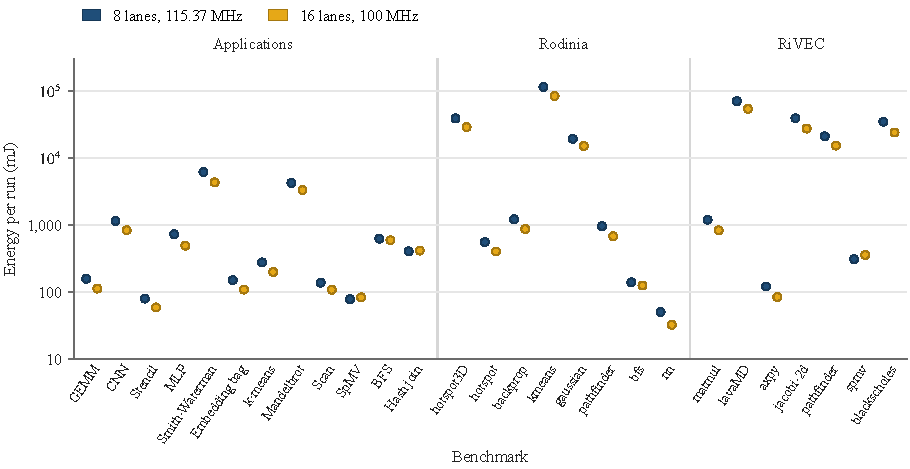
\includegraphics[width=\textwidth]{simtix_lanes_energy.pdf}
\caption{Energy per run of the eight- and 16-lane SIMTiX on the ZCU102.}
\label{fig:energy}
\end{figure*}

\section{Out-of-Context Comparison With Vortex}\label{sup:vortex}
\begin{table}[t]
\caption{SIMTiX and Vortex Out of Context}
\label{tab:vortex}
\centering\footnotesize
\setlength{\tabcolsep}{4pt}
\begin{tabular}{@{}lrrrr@{}}
\toprule
 & SIMTiX & \multicolumn{3}{c}{Vortex}\\
\cmidrule(lr){2-2}\cmidrule(lr){3-5}
 & 4 warps & 4 warps & 8 warps & 16 warps\\
\midrule
LUT            & 84,443 & 80,119 & 91,831 & 110,158\\
FF             & 31,959 & 78,613 & 86,452 & 98,570\\
BRAM           & 16     & 46     & 62     & 95.5\\
DSP            & 72     & 48     & 48     & 48\\
\Fmax\ (MHz)   & 101.6  & 140.8  & 135.9  & 134.0\\
Power (W)      & 1.10   & 1.70   & 1.85   & 2.08\\
\midrule
\multicolumn{5}{@{}l}{\emph{Vortex / SIMTiX, geometric mean over the seven applications}}\\
Warp instructions & --- & 1.72 & 1.72 & 1.73\\
Cycles         & --- & 2.78 & 1.80 & 1.58\\
Run time       & --- & 2.01 & 1.34 & 1.20\\
Energy         & --- & 4.32 & 3.04 & 3.00\\
\midrule
\multicolumn{5}{@{}l}{\emph{SIMTiX / Vortex, geometric mean}}\\
Performance per LUT  & --- & 1.90 & 1.46 & 1.57\\
Performance per watt & --- & 4.32 & 3.04 & 3.00\\
\bottomrule
\end{tabular}
\end{table}

To compare cost at equal configuration, we built SIMTiX and Vortex~3.0 with four warps
of eight threads and a 16~KiB L1, out of context with Vortex's own Vivado script at a
100~MHz constraint, and estimated their power vectorless at a toggle rate of 12.5\%.
Both run seven applications in simulation (GEMM, SpMV, a Jacobi stencil, k-means, BFS,
a prefix sum and an INT8 MLP), with the same algorithms and the same order of
floating-point operations, every output checked bit-exactly; Vortex's kernels are
compiled by its LLVM at \texttt{-O3}, and its simulator uses the FMA, divide and
square-root latencies of its IP cores (16, 28 and 28 cycles).

Table~\ref{tab:vortex} gives the results. Vortex executes 1.72 times the warp
instructions of SIMTiX (geometric mean), because its kernels carry divergence and
predicate instructions and compiled loop code, and the MLP has no INT8 dot product on
Vortex. With four warps it also reaches a lower IPC, 0.25 to 0.43 against SIMTiX's 0.43
to 0.69, because four warps do not fill its longer pipeline (Proposition~\ref{P-prop:ipc});
at 16 warps its IPC rises to 0.47--0.66, so most of its remaining cycle deficit comes
from its instruction count. Vortex closes at 140.8~MHz, 39\% above SIMTiX, and uses
5\% fewer LUTs but 2.5 times the flip-flops, 2.9 times the block RAM and 55\% more
power. Per LUT, SIMTiX delivers 1.46 to 1.90 times the performance of Vortex, and per
watt three to 4.3 times, at every Vortex warp count, with performance taken as the
inverse of the run time at each design's \Fmax, and at 100~MHz per watt.

Fig.~\ref{fig:vortex} gives, per application, the IPC, the execution time at each
design's \Fmax\ and the energy of one run at 100~MHz, from the vectorless power, of
SIMTiX with four warps and of Vortex with four, eight and 16 warps, from the
out-of-context builds of Section~\ref{P-sec:evalvortex} of the paper and Table~\ref{tab:vortex}.

Each application has one bar per design, on a log axis for the time and the energy.
SIMTiX is faster than Vortex with four warps on all seven applications and than Vortex
with 16 warps on five, all but GEMM and SpMV, and it uses the least energy on all seven.

\begin{figure*}[t]
\centering
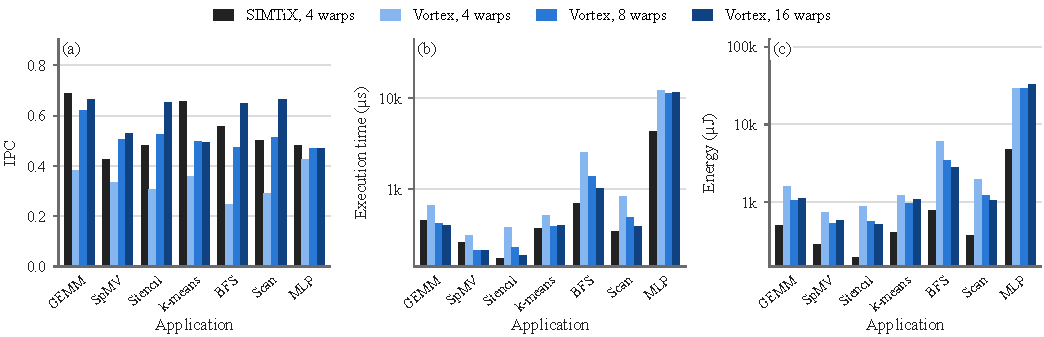
\includegraphics[width=\textwidth]{vortex_metrics.pdf}
\caption{SIMTiX and Vortex out of context. (a) IPC. (b) Execution time. (c) Energy.}
\label{fig:vortex}
\end{figure*}


\section{FGPU: Build, Kernels and Hardware Limits}\label{sup:fgpu}
FGPU~\cite{fgpu} is built from its public RTL with one compute unit (CU) of eight
processing elements (PEs), its floating-point units, regenerated for the XCZU9EG, and its
global atomics. A wavefront of 64 work-items issues one instruction over eight cycles, and
up to eight wavefronts are resident. FGPU is a peripheral of the A53 like the other
machines: an AXI4-Lite port for its control registers, kernel descriptor and code memory,
and a 64-bit AXI4 master to S\_AXI\_HP0. The board design closes at 187.48~MHz
($1.5$~GHz$/8$) with 1.02~ns of slack and uses 43,995 LUTs, 58,582 flip-flops, 49.5
RAMB36 and 64 DSP blocks; Vivado estimates 1.40~W for FGPU.

\emph{Kernels.} Every benchmark is written in OpenCL~C with one work-item per output,
reads the same parameter block as the SIMTiX kernel and keeps the operation order of the
definition; FGPU's LLVM~3.7 back end compiles it. FGPU has no fused multiply-add, no
conversion from float to integer, converts only unsigned integers to float and compares
floats only with ``less than''; the kernels multiply and add separately, round to an
integer and convert signed integers with the exact constant $1.5\cdot2^{23}$, and write
every comparison as $a<b$. Outputs that depend on a fused multiply-add of the definition
are checked within $10^{-3}$ of each row's largest reference value; the largest
difference on the board is $2.0\times10^{-4}$ (gaussian, whose elimination compounds
the separate roundings over 1,024 steps) and at most $1.7\times10^{-6}$ elsewhere. Where
the product is exact (the stencil's coefficient $1/8$, Mandelbrot's $2\,z_rz_i$ and its
pixel coordinates, multiples of $5\cdot2^{-k}$) the separate add equals the fused one and
the check stays exact. For the INT8 requantization the A53 reference multiplies and adds
separately on FGPU's runs, so its bytes stay exact. On kdd\_cup, k-means without fused
multiply-adds converges in the same 37 iterations to the same memberships and centers
(checked offline in IEEE single precision), so its exact check also holds.

\emph{Hardware limits.} Four properties of FGPU's hardware, each found in simulation of
its RTL or on the board, change the code of five benchmarks but not their outputs.
(i)~The atomic-add unit latches the address of the first atomic of a kernel and adds
there until the kernel ends; an atomic to another address is never retired, so the
kernel does not finish. k-means accumulates its cluster sums with atomics at
$3K$ addresses; on FGPU a first kernel assigns the points and adds to per-worker partial
sums in each worker's own memory words, and a second adds the partials.
(ii)~Byte and halfword stores are placed in their word only when FGPU is built with
sub-integer support, which its default configurations, and ours, leave out; otherwise
they write the whole word. MLP and CNN, whose outputs are bytes, compute four outputs
per work-item and store one word.
(iii)~Each work-item has 16 words of stack (FGPU's local memory, addressed by phase,
wavefront and a four-bit offset), and the compiler does not know the limit: lavaMD,
whose loop invariants the compiler keeps in registers and spills to an 18-word frame,
gave wrong forces on the board. Compiled without machine-level loop-invariant code
motion its frame is six words and its results are correct; the code of every other
RiVEC kernel is unchanged by the option.
(iv)~With several wavefronts in flight, a load that closely follows a store of the same
work-item to the same word can return the old value. The radix sort counts digits and
advances its scatter offsets in memory; on FGPU it keeps both in registers (16 packed
counters) and adds the digit bases in a kernel of its own. Pauses between kernels do not
change the failure, and k-means' partial sums, whose loads follow their stores by tens
of instructions, are correct.

Before the board, every kernel ran on FGPU's RTL in simulation (xsim, the board wrapper
and configuration) on the small inputs of the SIMTiX test suite and matched, bit for bit,
a single-precision model of the kernel; the model in turn reproduces the SIMTiX
reference within the tolerance above. Limits (iii) and (iv) appear only at board scale:
the small inputs put all lanes of a wavefront in one lavaMD box and give the sort about
one increment per counter.

% Material moved out of the paper in the focused rewrite of 2026-11-19
% (from simtix_tvlsi_long_2026-11-19.tex), included by simtix_tvlsi_supp.tex.

\section{Benchmark Rules and Changes}\label{sup:bench}
Each Rodinia benchmark is defined by Rodinia's computation on Rodinia's data: the
sequence of FP32 operations that produces one output, each rounded once, with a fused
multiply-add where the sum is fused. The input files are Rodinia's own. Work that
Rodinia performs on the CPU (the control of the bfs levels, the selection of the nearest
records in nn, the center update of kmeans and the back substitution of gaussian) runs
on the A53 for every machine and is not timed. For SIMTiX and Vortex, the A53's timer
measures from the first launch to the end of the last, including the host's work
between launches; for CVA6 and Ara, the cycle counter of CVA6 measures the kernel,
whose loop over iterations runs on CVA6 itself.

Three choices depart from Rodinia's default runs. All machines compute in FP32.
backprop uses 2$^{19}$ inputs rather than 2$^{21}$, whose two 256~MiB weight arrays do
not fit the memory region of the Ara host. gaussian uses the matrix that Rodinia
generates rather than its matrix file: Rodinia eliminates without pivoting, and on the
random matrix of the file the entries grow to $5.3\times10^{4}$, so that a change of one
ulp in 8.7\% of the quotients changes rows of the result by up to 6.3 times their
largest entry. This matters because the divide and square-root unit of CVA6, which Ara
shares, is not correctly rounded: on 4,096 random operands, 8.7\% of its quotients and
6.9\% of its square roots differ from the correctly rounded value by one ulp. Finally,
Ara computes gaussian's multipliers (Rodinia's Fan1 kernel, one division per row) on
CVA6, because its vector form returned wrong values, or deadlocked, when it ran after
nn; the elimination itself (Fan2) runs on Ara.

RiVEC computes in FP64; all machines here compute in FP32, the precision of SIMTiX and
Vortex. Each RiVEC application is defined by RiVEC's vector code read per element, with
RiVEC's fused multiply-adds and its polynomial exponential and logarithm; sums over many
elements (a row of spmv, the force on a particle in lavaMD) are defined in serial
order. SIMTiX, Vortex and CVA6 then produce the A53 reference bit for bit, and so does
Ara except in spmv and lavaMD, where its code keeps one partial sum per vector element
and reduces them at the end. blackscholes divides three times and takes one square root
per option; with the divide and square-root unit of CVA6, CVA6 and Ara give identical
prices that differ from the reference by up to $5.7\times10^{-4}$ of $|p|+0.01$. A model
of RiVEC's computation in which each quotient and square root is one ulp off at the
measured rates of 8.7\% and 6.9\% gives the same bound over 200 random trials on the
same options; the limit is $10^{-3}$.

RiVEC's code was changed in four places. Two are errors in RiVEC. Its blackscholes
negates the cumulative normal of the negative arguments with a masked subtract in the
mask-agnostic form, which allows an RVV~1.0 implementation to overwrite the unselected
elements; under QEMU, 46,277 of the 65,536 prices are wrong. We select the two results
with a merge instead. RiVEC's spmv builds the matrix from the file's column-major
entries with one-based indices and reads one element past the end of $x$; we use
zero-based indices, which computes $y=A^{\mathsf T}x$ for RiVEC's matrix. The other two
changes avoid faults of Ara. Ara reloads a vector register spilled to the stack with
wrong values, and GCC spills one in blackscholes, so RiVEC's code is compiled with
clang, which does not. Ara's jacobi-2d computed wrong last elements of some rows,
differently from run to run, when it ran after another kernel, while it reused vector
registers from one row to the next; it now loads the three rows for every output row,
which costs about 46\% more cycles in a reduced run.

\section{FP16 Arithmetic}\label{sup:fp16}
The FPU has five pipeline stages, and its 48-bit significand product is formed on a
$24\times24$ cascade of DSP blocks. FP16 operations widen their operands to FP32, use
the FP32 datapath and round the result to FP16, so an FP16 result is rounded twice. Let
$\circ_p$ denote rounding to nearest even and $\square_p$ rounding to odd, at $p$ bits
of significand: 24 for FP32, 11 for FP16.

\newtheorem{sproposition}{Proposition}
\renewcommand{\thesproposition}{S\arabic{sproposition}}
\begin{sproposition}
Let $x$ be the exact sum, difference, product, quotient or square root of FP16
operands, and $y=ab+c$ the exact result of an FMA of FP16 operands, with results in the
normal range of FP16. Then $\circ_{11}(\circ_{24}(x))=\circ_{11}(x)$ and
$\circ_{11}(\square_{24}(y))=\circ_{11}(y)$.
\end{sproposition}
\begin{IEEEproof}
For the five basic operations, double rounding to nearest is innocuous when the
intermediate precision $p$ and the target precision $q$ satisfy
$p\ge2q+2$~\cite{figueroa}; here $24=2\cdot11+2$. The exact result of an FMA is not the
result of such an operation on $q$-bit operands, so that bound does not apply. For any
real $y$, rounding to odd at $p\ge q+2$ bits followed by rounding to nearest at $q$
bits equals rounding to nearest at $q$ bits~\cite{boldo}, and $24\ge13$. FP32 contains
the exponent range of FP16, so neither rounding is affected by underflow or overflow
within the normal range.
\end{IEEEproof}

The FPU therefore rounds an FMA with an FP16 destination to odd at FP32 precision, and
its FP16 results in the default rounding mode are correctly rounded; the directed modes
are covered by the test vectors. We checked the units bit-exactly against an IEEE-754
reference~\cite{ieee754} on 116,089 arithmetic and 100,884 conversion vectors that
cover every rounding mode.

\section{Suite~2 and the Synchronization Kernels}\label{sup:suite2}
The board runs of Section~\ref{P-sec:lanes16} include a second suite of ten kernels,
\emph{suite~2}, drawn from five benchmark suites: pathfinder, hotspot and backprop from
Rodinia, Black-Scholes from RiVEC, PageRank and connected components from
GAP~\cite{gap}, the radix sort of SHOC~\cite{shoc}, and ATAX, BiCG and Jacobi-2D from
PolyBench~\cite{polybench}. Suite~2 follows the rules of the applications: each kernel
is defined by the sequence of FP32 operations of one output, SIMTiX runs hand-written
assembly, the A53 runs one C version and checks every output, and every kernel runs at
two input sizes. CVA6 and Ara also run suite~2 (Vortex has no ports of it); at the
larger input, the eight-lane SIMTiX is $14.6\times$ and $3.4\times$ faster than CVA6 and
Ara and the 16-lane SIMTiX $17.0\times$ and $4.0\times$ (geometric means), and Ara is
faster on Black-Scholes, whose results on CVA6 and Ara differ from SIMTiX's in the last
bits through their divider's rounding. FGPU also runs suite~2: the eight-lane SIMTiX is
$4.16\times$ faster at the larger input (geometric mean), from $2.05\times$ on hotspot to
$19.7\times$ on ATAX and BiCG, whose row-wise product gives each work-item of a wavefront
its own cache line at every step while FGPU fills two lines at a time, and
FGPU is faster on Black-Scholes (0.23 of SIMTiX's time), which divides.

\begin{figure*}[t]
\centering
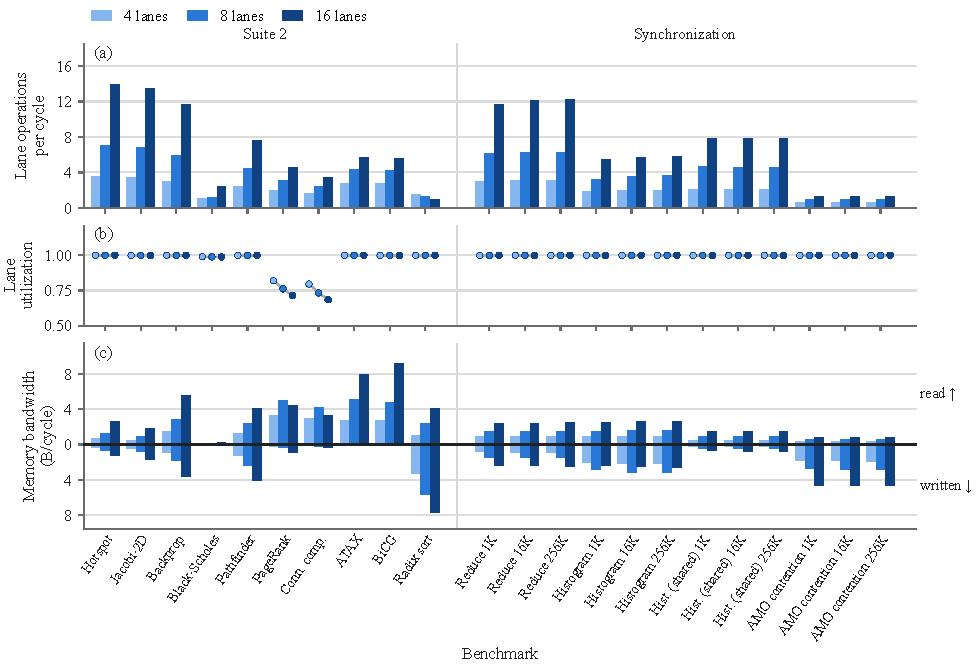
\includegraphics[width=\textwidth]{lanes_metrics_supp.pdf}
\caption{Throughput, lane utilization and memory bandwidth of suite~2 and the
synchronization kernels at 4, 8 and 16 lanes in simulation. (a) Lane operations per
cycle. (b) Lane utilization. (c) Bytes read (up) and written (down) per cycle.}
\label{fig:lanes_s2sync}
\end{figure*}

Fig.~\ref{fig:lanes_s2sync} completes the lane-scaling study of
Section~\ref{P-sec:evallanes} of the paper; the synchronization kernels run at 1K, 16K
and 256K threads. At four, eight and 16 lanes, the geometric-mean throughput is 2.24,
3.49 and 5.33 lane operations per cycle for suite~2, with a lane utilization of 0.96,
0.94 and 0.93, and 1.68, 3.09 and 5.12 for the synchronization kernels, whose lanes
never diverge. The utilization of PageRank and connected components falls from 0.82
and 0.80 at four lanes to 0.71 and 0.69 at 16, for the reason given for BFS in the
paper. Black-Scholes is flat from four to eight
lanes and $2\times$ at 16 (one divide/square-root unit below 16 lanes). The block-shared
histogram gains $2.2\times$ from four to eight lanes: at four lanes its 32-thread blocks
take all eight warps, so each block barrier stalls the whole machine. Radix sort slows
as lanes are added ($0.90\times$ and $0.67\times$), because its scattered stores move
lines of one word per lane: its write traffic rises from 3.3 to 7.7 bytes per cycle
while its throughput falls. ATAX and BiCG read the most, 7.9 and 9.1 bytes per cycle at
16 lanes, of the 16 the port carries. At four lanes, the eight-thread groups of the AMO-contention
kernel span two warps whose order is not defined, so its check covers the results that
do not depend on that order: every \texttt{amoadd} sum and every \texttt{amomax}
maximum, which a lost update would change.

\section{Throughput Against the Peak}\label{sup:lanestp}
Tables~\ref{tab:lanes_tp} and~\ref{tab:lanes_cyc} give the useful throughput and the
cycles of 15 applications at 4, 8 and 16 lanes in simulation, with one 64~KiB L1 and one
divide/square-root unit at every lane count, eight warps, 16 MSHRs, 16 tags and an AXI4
memory model of 24 cycles, every output checked. The \emph{throughput} counts only the
useful operations: FP32 operations, with an FMA counted as two; INT8
multiply-accumulates for the CNN and the MLP; and lane operations, the issued warp
instructions times their active lanes, for the integer kernels. The \emph{ideality} is
the throughput divided by the peak, $2L$ FLOP, $4L$ MAC or $L$ lane operations per
cycle, and the speedup of a doubling is the ratio of the cycles before and after it. The compute kernels gain 1.93 to $2.05\times$ per doubling at constant IPC and
ideality; their ideality is set by the instructions that compute addresses and control
loops: 0.14 for GEMM against 0.47 for the register-blocked GEMM-RB. The gather kernels
gain 1.27 to $1.60\times$ per doubling, and their IPC falls, from 0.73 to 0.39 for
SpMV-Z.

\begin{table*}[t]
\caption{Throughput and Ideality at 4, 8 and 16 Lanes}
\label{tab:lanes_tp}
\centering\footnotesize
\setlength{\tabcolsep}{4.5pt}
\begin{tabular}{llrrrrrr}
\toprule
Kernel (board input) & Metric & \multicolumn{3}{c}{Throughput} & \multicolumn{3}{c}{Ideality}\\
\cmidrule(lr){3-5}\cmidrule(lr){6-8}
 & & 4 lanes & 8 lanes & 16 lanes & 4 & 8 & 16\\
\midrule
GEMM ($n=128$)             & FLOP/cycle    & 1.08 & 2.17 & 4.36           & 0.14 & 0.14 & 0.14\\
GEMM-RB ($n=128$)          & FLOP/cycle    & 3.80 & 7.63 & \textbf{14.86} & 0.47 & 0.48 & 0.46\\
Stencil ($128^2$)          & FLOP/cycle    & 0.61 & 1.22 & 2.40           & 0.08 & 0.08 & 0.08\\
Stencil-RB ($128^2$)       & FLOP/cycle    & 1.34 & 2.63 & 5.09           & 0.17 & 0.16 & 0.16\\
Embedding bag (256 bags)   & FLOP/cycle    & 0.43 & 0.88 & 1.76           & 0.05 & 0.05 & 0.05\\
SpMV (4096 rows)           & FLOP/cycle    & 0.31 & 0.49 & 0.69           & 0.04 & 0.03 & 0.02\\
SpMV-Z (4096 rows)         & FLOP/cycle    & 0.38 & 0.56 & 0.71           & 0.05 & 0.03 & 0.02\\
CNN, INT8 ($32^2$)         & MAC/cycle     & 3.36 & 6.74 & \textbf{13.46} & 0.21 & 0.21 & 0.21\\
MLP, INT8 (batch 16)       & MAC/cycle     & 1.36 & 2.71 & 5.31           & 0.08 & 0.08 & 0.08\\
k-means (16k points)       & lane-op/cycle & 3.40 & 6.77 & \textbf{13.43} & 0.85 & 0.85 & 0.84\\
k-means-U (16k points)     & lane-op/cycle & 3.41 & 6.67 & 12.31          & 0.85 & 0.83 & 0.77\\
BFS (16k vertices)         & lane-op/cycle & 1.59 & 2.36 & 3.41           & 0.40 & 0.30 & 0.21\\
Scan (64k elements)        & lane-op/cycle & 2.73 & 5.11 & 9.26           & 0.68 & 0.64 & 0.58\\
Segmented scan (64k)       & lane-op/cycle & 2.65 & 5.48 & 11.03          & 0.66 & 0.68 & 0.69\\
Hash join (16k probes)     & lane-op/cycle & 2.00 & 2.98 & 3.98           & 0.50 & 0.37 & 0.25\\
\bottomrule
\end{tabular}

\end{table*}

\begin{table*}[t]
\caption{Cycles, IPC and Speedup From Doubling the Lanes}
\label{tab:lanes_cyc}
\centering\footnotesize
\setlength{\tabcolsep}{4.5pt}
\begin{tabular}{lrrrrrrrr}
\toprule
Kernel & \multicolumn{3}{c}{Cycles} & \multicolumn{3}{c}{IPC} & \multicolumn{2}{c}{Speedup}\\
\cmidrule(lr){2-4}\cmidrule(lr){5-7}\cmidrule(lr){8-9}
 & 4 lanes & 8 lanes & 16 lanes & 4 & 8 & 16 & $4\to8$ & $8\to16$\\
\midrule
GEMM           & 3,880,530 & 1,933,322 & 962,975   & 0.97 & 0.97 & 0.98 & $2.01\times$ & $2.01\times$\\
GEMM-RB        & 1,104,255 & 549,599   & 282,239   & 0.94 & 0.94 & 0.91 & $2.01\times$ & $1.95\times$\\
Stencil        & 645,220   & 323,558   & 163,509   & 0.84 & 0.84 & 0.83 & $1.99\times$ & $1.98\times$\\
Stencil-RB     & 293,823   & 149,285   & 77,252    & 0.83 & 0.81 & 0.79 & $1.97\times$ & $1.93\times$\\
Embedding bag  & 306,918   & 149,493   & 74,476    & 0.77 & 0.79 & 0.79 & $2.05\times$ & $2.01\times$\\
CNN (INT8)     & 4,213,951 & 2,100,529 & 1,051,662 & 0.75 & 0.75 & 0.75 & $2.01\times$ & $2.00\times$\\
MLP (INT8)     & 2,778,021 & 1,388,607 & 709,769   & 0.70 & 0.70 & 0.68 & $2.00\times$ & $1.96\times$\\
k-means        & 1,683,383 & 844,828   & 425,681   & 0.85 & 0.85 & 0.84 & $1.99\times$ & $1.98\times$\\
k-means-U      & 1,049,558 & 536,692   & 290,751   & 0.85 & 0.83 & 0.77 & $1.96\times$ & $1.85\times$\\
Segmented scan & 511,400   & 282,781   & 158,199   & 0.66 & 0.69 & 0.69 & $1.81\times$ & $1.79\times$\\
Scan           & 1,436,259 & 813,498   & 483,430   & 0.72 & 0.68 & 0.61 & $1.77\times$ & $1.68\times$\\
SpMV           & 209,987   & 131,585   & 94,319    & 0.77 & 0.68 & 0.50 & $1.60\times$ & $1.40\times$\\
BFS            & 1,667,225 & 1,121,490 & 776,421   & 0.71 & 0.67 & 0.59 & $1.49\times$ & $1.44\times$\\
Hash join      & 270,265   & 181,411   & 135,937   & 0.71 & 0.66 & 0.54 & $1.49\times$ & $1.33\times$\\
SpMV-Z         & 170,211   & 116,877   & 91,978    & 0.73 & 0.58 & 0.39 & $1.46\times$ & $1.27\times$\\
\bottomrule
\end{tabular}

\end{table*}

\section{Simulated Applications and Timing Closure}\label{sup:sim}
\begin{table}[t]
\caption{Applications and Their Inputs}
\label{tab:apps}
\centering\footnotesize
\setlength{\tabcolsep}{2.6pt}
\begin{tabular}{llrrrrl}
\toprule
App. & Simulated input & Cycles & IPC & Util. & L1 hit & Board input\\
\midrule
GEMM    & $32^3$               & 45,902  & 0.69 & 100\% & 93\% & $256^3$\\
SpMV    & $512^2$, $\le$16/row & 26,295  & 0.43 & 59\%  & 88\% & $65{,}536^2$\\
Stencil & $32^2$, 2 sweeps     & 17,529  & 0.48 & 100\% & 88\% & $512^2$, 4\\
k-means & 1,024, $k=8$         & 36,935  & 0.66 & 100\% & 93\% & $2^{18}$, 16\\
BFS     & 1,024, degree 6      & 71,151  & 0.56 & 43\%  & 84\% & $2^{18}$, 8\\
Scan    & 2,048                & 34,468  & 0.50 & 95\%  & 73\% & $2^{20}$\\
MLP     & 784-128-10, 8        & 433,626 & 0.48 & 100\% & 50\% & 3 layers, 256\\
\bottomrule
\end{tabular}

\end{table}

Table~\ref{tab:apps} lists the seven applications of the simulation studies of
Sections~\ref{P-sec:evalamo} and~\ref{P-sec:evalvortex} of the paper, with their
cycles, IPC, lane utilization (Util.: the active lanes of the issued warp instructions
over eight times their number) and L1 read hit rate. They are written
in RISC-V assembly with one thread per output: FP32 matrix multiplication, sparse
matrix-vector product in compressed sparse row format, two sweeps of a five-point
Jacobi stencil, the assignment step of k-means with AMO accumulation of the cluster
sums, level-synchronous breadth-first search with one launch per level and an
\texttt{amoor} flag, an inclusive prefix sum built from a block scan with shuffles,
block-shared memory and a barrier, and a two-layer INT8 multilayer perceptron with
\texttt{pdot8}, requantization and a rectified linear unit.

On the board (Table~\ref{P-tab:board} of the paper) the twelve applications run at
large inputs: hash join with $2^{22}$ slots and $2^{20}$ probes; CNN on $128^2$ with
16-32-32 channels; GEMM $256^3$; embedding bag with $2^{18}$ rows of 32 floats and 4,096
bags of 32; BFS on $2^{18}$ vertices; SpMV with 65,536 rows; Mandelbrot $1024^2$ with 256
iterations; Smith-Waterman on 16,384 pairs of 32 and 128 bases; k-means with $2^{18}$
points and 16 clusters; stencil $512^2$ with four sweeps; MLP 784-256-128-10 with a batch
of 256; and scan of $2^{20}$ elements.

\emph{Timing closure.} Adding the L1 and the aggregated AMOs to the board design first
missed 100~MHz by 2.478~ns with 16,301 failing endpoints. The worst path was a
single-cycle loop of 30 logic levels, 76\% of it routing, from the pending-lane masks of
a memory context through port arbitration and address selection into the L1 tag
compare, the hit, the completion of the context and the warp's resume into its
reconvergence stack. Four changes closed it: the L1 registers its input; a context
completes from registered state and the cycle's responses; the L1 chooses one cycle
ahead which waiting read it answers next; and a post-route physical optimization pass.
The input register costs 1.5--2.5\% of the applications' cycles. In the routed
four-warp design, 38,680 endpoints failed at 150~MHz, 12,087 at 125~MHz and about 2,455
at 111~MHz, in four groups: warp issue into the memory engine's context registers, warp
issue into the reconvergence stack, the memory engine's request choice into the L1 input
register, and the first and last stages of the lane FPUs. Reaching 150~MHz would need an
operand-read stage across the whole issue logic, so we cut the four groups instead.


\section{Sixteen Lanes on the Board, Every Run}\label{sup:lanes16}
Tables~\ref{tab:lanes16_board_all1} and~\ref{tab:lanes16_board_all2} list the 82
board runs of Section~\ref{P-sec:lanes16} of the paper, summarized in
Table~\ref{P-tab:lanes16_board}: the time of the
Cortex-A53, of the eight-lane design and of the 16-lane design, and the 16-lane design's
speedup in time and in cycles over the eight-lane design and over the A53. The
eight-lane runs use their own A53 times, measured in the same session, and the A53 runs
the \texttt{-O2} reference. The input is each benchmark's size argument (elements,
matrix order, grid side or iterations); slower runs are in italics.

% generated by sim/compare_board_l16.py from the board logs (2026-11-17)
\begin{table*}[p]
\caption{Sixteen Lanes on the Board: Synchronization Kernels and Applications}
\label{tab:lanes16_board_all1}
\centering\footnotesize
\setlength{\tabcolsep}{4pt}
\begin{tabular}{lrrrrrrrr}
\toprule
Kernel & Input & \multicolumn{3}{c}{Time (ms)} & \multicolumn{2}{c}{16L vs 8L} & \multicolumn{2}{c}{vs A53}\\
\cmidrule(lr){3-5}\cmidrule(lr){6-7}\cmidrule(lr){8-9}
 & & A53 & 8 lanes & 16 lanes & time & cycles & 8L & 16L\\
\midrule
\multicolumn{9}{l}{\textit{Synchronization kernels}}\\
Reduce (shuffle) & 1{,}024 & 0.002 & 0.025 & 0.017 & 1.44 & 1.67 & 0.08 & 0.12\\
Histogram (AMO) & 1{,}024 & 0.008 & 0.025 & 0.019 & 1.28 & 1.51 & 0.33 & 0.43\\
Histogram (shared) & 1{,}024 & 0.008 & 0.039 & 0.028 & 1.38 & 1.61 & 0.21 & 0.29\\
AMO contention & 1{,}024 & 0.021 & 0.148 & 0.125 & 1.18 & 1.37 & 0.15 & 0.17\\
Reduce (shuffle) & 16{,}384 & 0.027 & 0.374 & 0.254 & 1.47 & 1.70 & 0.07 & 0.11\\
Histogram (AMO) & 16{,}384 & 0.125 & 0.352 & 0.273 & 1.29 & 1.49 & 0.36 & 0.46\\
Histogram (shared) & 16{,}384 & 0.125 & 0.638 & 0.427 & 1.50 & 1.73 & 0.20 & 0.29\\
AMO contention & 16{,}384 & 0.352 & 2.32 & 1.98 & 1.17 & 1.35 & 0.15 & 0.18\\
Reduce (shuffle) & 262{,}144 & 0.432 & 5.95 & 4.04 & 1.47 & 1.70 & 0.07 & 0.11\\
Histogram (AMO) & 262{,}144 & 2.00 & 5.65 & 4.34 & 1.30 & 1.51 & 0.35 & 0.46\\
Histogram (shared) & 262{,}144 & 2.00 & 10.26 & 6.78 & 1.51 & 1.74 & 0.19 & 0.29\\
AMO contention & 262{,}144 & 6.18 & 37.20 & 31.70 & 1.17 & 1.35 & 0.17 & 0.20\\
\midrule
\multicolumn{9}{l}{\textit{Applications}}\\
GEMM & 64 & 2.69 & 2.17 & 1.24 & 1.75 & 2.02 & 1.25 & 2.17\\
GEMM & 256 & 170 & 151 & 85.36 & 1.77 & 2.04 & 1.13 & 1.99\\
SpMV & 4{,}096 & 0.479 & 1.14 & 0.935 & 1.22 & 1.40 & 0.42 & 0.51\\
SpMV & 65{,}536 & 18.29 & 20.24 & 18.63 & 1.09 & 1.25 & 0.90 & 0.98\\
Stencil & 128 & 1.34 & 2.73 & 1.59 & 1.72 & 1.99 & 0.48 & 0.85\\
Stencil & 512 & 22.02 & 43.56 & 25.26 & 1.72 & 1.99 & 0.49 & 0.87\\
k-means & 16{,}384 & 2.58 & 7.26 & 4.23 & 1.72 & 1.98 & 0.36 & 0.61\\
k-means & 262{,}144 & 41.32 & 116 & 67.19 & 1.73 & 1.99 & 0.36 & 0.62\\
BFS & 16{,}384 & 4.37 & 9.38 & 7.42 & 1.27 & 1.46 & 0.47 & 0.59\\
BFS & 262{,}144 & 196 & 163 & 132 & 1.23 & 1.42 & 1.20 & 1.48\\
Scan & 65{,}536 & 0.284 & 6.76 & 4.60 & 1.47 & 1.70 & 0.04 & 0.06\\
Scan & 1{,}048{,}576 & 4.54 & 108 & 73.40 & 1.47 & 1.70 & 0.04 & 0.06\\
MLP{,} INT8 & 16 & 46.17 & 11.85 & 6.60 & 1.80 & 2.07 & 3.89 & 7.00\\
MLP{,} INT8 & 256 & 730 & 190 & 105 & 1.80 & 2.08 & 3.85 & 6.94\\
GEMM-RB & 64 & 2.70 & 0.603 & 0.365 & 1.65 & 1.91 & 4.48 & 7.40\\
GEMM-RB & 256 & 170 & 37.73 & 21.91 & 1.72 & 1.99 & 4.50 & 7.74\\
Segmented scan & 65{,}536 & 0.284 & 2.23 & 1.43 & 1.56 & 1.80 & 0.13 & 0.20\\
Segmented scan & 1{,}048{,}576 & 4.54 & 35.48 & 22.84 & 1.55 & 1.79 & 0.13 & 0.20\\
Stencil-RB & 128 & 1.36 & 1.20 & 0.721 & 1.66 & 1.92 & 1.10 & 1.88\\
Stencil-RB & 512 & 22.04 & 18.95 & 10.99 & 1.72 & 1.99 & 1.12 & 2.01\\
k-means-U & 16{,}384 & 2.58 & 4.56 & 2.81 & 1.62 & 1.87 & 0.57 & 0.92\\
k-means-U & 262{,}144 & 41.35 & 72.16 & 42.11 & 1.71 & 1.98 & 0.57 & 0.98\\
SpMV-Z & 4{,}096 & 0.477 & 1.01 & 0.914 & 1.11 & 1.28 & 0.47 & 0.52\\
SpMV-Z & 65{,}536 & 18.25 & 19.34 & 18.50 & 1.05 & 1.21 & 0.94 & 0.99\\
CNN{,} INT8 & 32 & 74.48 & 18.21 & 10.52 & 1.73 & 2.00 & 4.09 & 7.08\\
CNN{,} INT8 & 128 & 1{,}192 & 291 & 167 & 1.74 & 2.01 & 4.10 & 7.13\\
Embedding bag & 256 & 2.05 & 1.28 & 0.732 & 1.74 & 2.01 & 1.61 & 2.80\\
Embedding bag & 4{,}096 & 68.90 & 37.45 & 21.44 & 1.75 & 2.02 & 1.84 & 3.21\\
Hash join & 16 & 1.67 & 1.54 & 1.25 & 1.24 & 1.43 & 1.07 & 1.33\\
Hash join & 22 & 195 & 99.28 & 82.38 & 1.21 & 1.39 & 1.97 & 2.37\\
Mandelbrot & 256 & 53.00 & 68.27 & 42.40 & 1.61 & 1.86 & 0.78 & 1.25\\
Mandelbrot & 1{,}024 & 847 & 1{,}020 & 609 & 1.67 & 1.93 & 0.83 & 1.39\\
Smith-Waterman & 2{,}048 & 129 & 202 & 116 & 1.73 & 2.00 & 0.57 & 1.10\\
Smith-Waterman & 16{,}384 & 1{,}028 & 1{,}613 & 931 & 1.73 & 2.00 & 0.57 & 1.10\\
\bottomrule
\end{tabular}

\end{table*}

\begin{table*}[p]
\caption{Sixteen Lanes on the Board: Suite 2, Rodinia and RiVEC}
\label{tab:lanes16_board_all2}
\centering\footnotesize
\setlength{\tabcolsep}{4pt}
\begin{tabular}{lrrrrrrrr}
\toprule
Kernel & Input & \multicolumn{3}{c}{Time (ms)} & \multicolumn{2}{c}{16L vs 8L} & \multicolumn{2}{c}{vs A53}\\
\cmidrule(lr){3-5}\cmidrule(lr){6-7}\cmidrule(lr){8-9}
 & & A53 & 8 lanes & 16 lanes & time & cycles & 8L & 16L\\
\midrule
\multicolumn{9}{l}{\textit{Suite 2}}\\
Pathfinder & 65{,}536 & 69.76 & 165 & 101 & 1.64 & 1.89 & 0.42 & 0.69\\
Pathfinder & 262{,}144 & 275 & 659 & 402 & 1.64 & 1.89 & 0.42 & 0.68\\
Hotspot & 512 & 37.46 & 55.79 & 32.16 & 1.73 & 2.00 & 0.66 & 1.16\\
Hotspot & 1{,}024 & 152 & 223 & 130 & 1.72 & 1.99 & 0.68 & 1.17\\
Jacobi-2D & 512 & 46.56 & 84.14 & 48.96 & 1.72 & 1.98 & 0.54 & 0.95\\
Jacobi-2D & 2{,}048 & 782 & 1{,}351 & 787 & 1.72 & 1.98 & 0.58 & 0.99\\
ATAX & 1{,}024 & 15.16 & 19.86 & 18.65 & 1.06 & 1.23 & 0.76 & 0.81\\
ATAX & 4{,}096 & 243 & 356 & 401 & \textit{0.89} & 1.03 & 0.68 & 0.61\\
BiCG & 1{,}024 & 15.16 & 19.93 & 17.47 & 1.14 & 1.32 & 0.76 & 0.87\\
BiCG & 4{,}096 & 243 & 357 & 408 & \textit{0.88} & 1.01 & 0.68 & 0.60\\
PageRank & 16{,}384 & 25.07 & 33.35 & 25.83 & 1.29 & 1.49 & 0.75 & 0.97\\
PageRank & 262{,}144 & 909 & 649 & 842 & \textit{0.77} & 0.89 & 1.40 & 1.08\\
Connected comp. & 16{,}384 & 16.82 & 30.94 & 22.31 & 1.39 & 1.60 & 0.62 & 0.75\\
Connected comp. & 262{,}144 & 801 & 623 & 749 & \textit{0.83} & 0.96 & 1.29 & 1.07\\
Backprop & 65{,}536 & 26.80 & 37.42 & 21.71 & 1.72 & 1.99 & 0.71 & 1.23\\
Backprop & 524{,}288 & 215 & 299 & 174 & 1.72 & 1.99 & 0.72 & 1.24\\
Radix sort & 65{,}536 & 16.16 & 65.23 & 100 & \textit{0.65} & 0.75 & 0.25 & 0.16\\
Radix sort & 1{,}048{,}576 & 273 & 1{,}026 & 1{,}584 & \textit{0.65} & 0.75 & 0.27 & 0.17\\
Black-Scholes & 65{,}536 & 27.06 & 112 & 64.60 & 1.73 & 2.00 & 0.24 & 0.42\\
Black-Scholes & 1{,}048{,}576 & 438 & 1{,}790 & 1{,}033 & 1.73 & 2.00 & 0.24 & 0.42\\
\midrule
\multicolumn{9}{l}{\textit{Rodinia}}\\
Pathfinder & 100{,}000 & 97.12 & 250 & 153 & 1.64 & 1.89 & 0.39 & 0.63\\
Backprop & 524{,}288 & 214 & 299 & 174 & 1.72 & 1.99 & 0.72 & 1.23\\
BFS & 65{,}536 & 21.91 & 36.68 & 27.98 & 1.31 & 1.51 & 0.60 & 0.78\\
Hotspot & 512 & 21.00 & 33.55 & 19.34 & 1.74 & 2.00 & 0.63 & 1.09\\
Hotspot & 1{,}024 & 85.47 & 134 & 77.28 & 1.74 & 2.00 & 0.64 & 1.11\\
NN & 42{,}764 & 1.04 & 15.29 & 8.82 & 1.73 & 2.00 & 0.07 & 0.12\\
Hotspot3D & 512 & 16{,}561 & 9{,}450 & 5{,}472 & 1.73 & 1.99 & 1.75 & 3.03\\
Gaussian & 1{,}024 & 3{,}917 & 4{,}965 & 3{,}324 & 1.49 & 1.72 & 0.79 & 1.18\\
k-means & 494{,}020 & 28{,}065 & 31{,}810 & 18{,}163 & 1.75 & 2.02 & 0.88 & 1.55\\
\midrule
\multicolumn{9}{l}{\textit{RiVEC}}\\
AXPY & 2{,}097{,}152 & 25.04 & 31.49 & 18.00 & 1.75 & 2.02 & 0.80 & 1.39\\
Matmul & 512 & 2{,}153 & 300 & 172 & 1.75 & 2.02 & 7.17 & 12.54\\
SpMV & 85{,}623 & 52.75 & 79.22 & 84.02 & \textit{0.94} & 1.09 & 0.67 & 0.63\\
Jacobi-2D & 256 & 4{,}461 & 10{,}117 & 5{,}846 & 1.73 & 2.00 & 0.44 & 0.76\\
Pathfinder & 2{,}048 & 2{,}298 & 5{,}557 & 3{,}523 & 1.58 & 1.86 & 0.45 & 0.65\\
Black-Scholes & 65{,}536 & 3{,}454 & 9{,}328 & 5{,}394 & 1.73 & 2.00 & 0.37 & 0.64\\
LavaMD & 1{,}000 & 23{,}439 & 15{,}868 & 9{,}152 & 1.73 & 2.00 & 1.48 & 2.56\\
\bottomrule
\end{tabular}

\end{table*}



\section{Memory System and Reduction in the v2 Design}\label{sup:evalmem}
We measured the L1 and the memory contexts as they were added, with a set of
synchronization kernels and a memory model of fixed latency. With a 20-cycle
memory, the L1 makes a 16-bin histogram $5.6\times$ faster, its block-shared form
$2.4\times$ and a whole-array sum (a shuffle butterfly and one AMO per warp)
$1.5\times$, while reductions that read each line once change by less than 5\%.
With a 7-cycle memory, four contexts instead of one reduce the cycles of the
whole-array sum by 15\% and of the histogram by 14\%.

In our earlier design without shuffles, a reduction of 1,024 values to one sum
per warp took 6,023 cycles through the scratchpad, 1.38 times the 4,363 cycles of
the same computation on a five-stage RV32I core at the same clock with
single-cycle memory. With a butterfly of three \texttt{shfl.xor} steps, which
leaves the sum in every lane, the reduction takes 2,911 cycles, 1.50 times faster
than that core, and 3,908 cycles behind the L1 and the AXI4 memory model.



\section{Instruction Sets}\label{sup:isa}
Table~\ref{tab:isa} places the SIMTiX instruction set beside the GPU instruction sets
compared in~\cite{vortex} (Table~1 there); Section~\ref{P-sec:related} of the paper
discusses the differences. GDS and LDS are the global and local data shares, VGPR and
SGPR the vector and scalar general-purpose registers, CTA a cooperative thread array,
GRF the general register file, SPF a special flag and USC the unified shading cluster.

\begin{table*}[t]
\caption{GPU Instruction Sets and SIMTiX}
\label{tab:isa}
\centering\scriptsize
\setlength{\tabcolsep}{2.2pt}
\renewcommand{\arraystretch}{1.15}
\begin{tabular}{l*{9}{>{\raggedright\arraybackslash}p{0.087\textwidth}}}
\toprule
ISA & Memory model & Threading model & Register file & Thread control &
Synchro\-nization & Flow control & ALU operations & Memory operations & GPU operations\\
\midrule
RDNA & GDS, LDS, constants, global & Workgroup, wavefront, 32/64 threads &
Vector/scalar, 256 VGPRs, 106 SGPRs & End threads, thread mask &
Barrier, wait\_cnt, data dep. & Branch, thread mask & Arithmetic, conditional, bitwise &
Load, store, prefetch & Interpolate, texture sampler\\
GCN & GDS, LDS, constants, global & Compute unit, wavefront, 64 threads &
Vector/scalar, 256 VGPRs, 102 SGPRs & End threads, thread mask &
Barrier, wait\_cnt, data dep. & Branch, thread mask, split/join &
Arithmetic, conditional, bitwise & Load, store, prefetch & Interpolate, texture sampler\\
PTX & Shared, texture, constants, global & Grid/CTA, warp, 32 threads & Scalar &
Predicate & Barrier, membar & Branch, predicate & Arithmetic, conditional, bitwise &
Load, store, prefetch & Texture sampler, load, query\\
GEN & Software managed & Root thread, child thread &
256-bit vector, 128 GRFs, predicate & Send message & Wait, fence &
Branch, SPF registers, split/join & Arithmetic, conditional, bitwise & Load, store &
Interpolate, texture sampler\\
PowerVR & Global, common store, unified store & USC, 32 threads & Vector, 128-bit &
Predicate & Fence & Branch, predicate & Arithmetic, conditional, bitwise & Load, store &
Texture sampler, iteration, alpha/depth\\
Vortex & Shared, global & Compute unit, wavefront & Scalar, 32-bit & Thread mask &
Barrier, flush & Split/join & Arithmetic, conditional, bitwise & Load, store &
Texture sampler\\
\midrule
SIMTiX & Global (L1), block-shared, warp-private & Kernel, block of $2^b$ warps, warp
of 8 threads & Scalar, 32-bit, 32 integer + 32 FP & Hardware spawn, \texttt{ecall},
thread mask & Barrier (\texttt{bar}), RV32A AMOs & Branch, hardware reconvergence
stack & Arithmetic, conditional, bitwise, FP32/FP16, Zba, Zbb min/max, Zicond &
Load, store, line-aggregated AMOs & Shuffle, INT8 dot product (\texttt{pdot8})\\
\bottomrule
\end{tabular}

\end{table*}


\begin{thebibliography}{9}
\bibitem{fgpu} M.~Al~Kadi, B.~Janssen, and M.~H\"ubner, ``FGPU: An
SIMT-architecture for FPGAs,'' in \emph{Proc. ACM/SIGDA Int. Symp.
Field-Programmable Gate Arrays (FPGA)}, 2016, pp.~254--263.
\bibitem{vortex} B.~Tine, K.~P.~Yalamarthy, F.~Elsabbagh, and H.~Kim,
``Vortex: Extending the RISC-V ISA for GPGPU and 3D-graphics,'' in
\emph{Proc. IEEE/ACM Int. Symp. Microarchitecture (MICRO)}, 2021, pp.~754--766.
\bibitem{figueroa} S.~A.~Figueroa, ``When is double rounding innocuous?''
\emph{ACM SIGNUM Newsl.}, vol.~30, no.~3, pp.~21--26, 1995.
\bibitem{boldo} S.~Boldo and G.~Melquiond, ``Emulation of FMA and correctly rounded
sums: Proved algorithms using rounding to odd,'' \emph{IEEE Trans. Comput.}, vol.~57,
no.~4, pp.~462--471, Apr. 2008.
\bibitem{ieee754} \emph{IEEE Standard for Floating-Point Arithmetic}, IEEE Std
754-2019, 2019.
\bibitem{gap} S.~Beamer, K.~Asanovi\'c, and D.~Patterson, ``The GAP benchmark suite,''
arXiv:1508.03619, 2015.
\bibitem{shoc} A.~Danalis, G.~Marin, C.~McCurdy, J.~S.~Meredith, P.~C.~Roth, K.~Spafford,
V.~Tipparaju, and J.~S.~Vetter, ``The Scalable Heterogeneous Computing (SHOC) benchmark
suite,'' in \emph{Proc. 3rd Workshop General-Purpose Comput. Graph. Process. Units
(GPGPU-3)}, 2010, pp.~63--74.
\bibitem{polybench} L.-N.~Pouchet, ``PolyBench/C: The polyhedral benchmark suite,''
2012. [Online]. Available: \url{https://sourceforge.net/projects/polybench/}
\end{thebibliography}

\end{document}
